\documentclass[conference]{IEEEtran}

% *** MISC UTILITY PACKAGES ***
%


% *** CITATION PACKAGES ***
%
\usepackage{cite}

% *** GRAPHICS RELATED PACKAGES ***
%
\usepackage[pdftex]{graphicx}
% declare the path(s) where your graphic files are
\graphicspath{{./images/}}
\DeclareGraphicsExtensions{.pdf,.jpeg,.png}

% *** MATH PACKAGES ***
%
\usepackage[cmex10]{amsmath}

% *** SPECIALIZED LIST PACKAGES ***
%
%\usepackage{algorithmic}
\usepackage{algpseudocode}
% *** ALIGNMENT PACKAGES ***
%
\usepackage{array}


% *** SUBFIGURE PACKAGES ***
\usepackage[cpation=false,font=footnotesize]{subfig}

% *** FLOAT PACKAGES ***
%

% *** PDF, URL AND HYPERLINK PACKAGES ***
%
\usepackage{url}


% correct bad hyphenation here
\hyphenation{}


\begin{document}
%
% paper title
\title{Wall following and obstacle avoidance with SARSA $\lambda$}


% author names and affiliations
\author{\IEEEauthorblockN{Matthew J. Urffer}
\IEEEauthorblockA{
University of Tennessee \\
Knoxville, Tennessee, 37916 \\
Email: matthew.urffer@gmail.com
}}



% make the title area
\maketitle


\begin{abstract}
\boldmath
Reinforcement learning is a learning process in which an agent is reward for making the correct actions at a particular state. 
This learning strategy is extremely useful in complex environments that are difficult to modeled, or ones in which the easement of an action is delayed.
This work attempts to implement a reinforcement learning strategy for a wall-following and obstacle avoidance robot in the player stage environment.
Attempts were made to implement reinforcement learning using the SARSA $\lambda$ algorithm with an $\epsilon$ greedy policy and eligibility traces, but ultimately these attempts did not result in a convergent implementation.
In this implementation a discredited state space was utilized as well as a discrete action space.
\end{abstract}
\IEEEpeerreviewmaketitle



\section{Introduction}

Reinforcement learning is a popular learning strategy for which direct supervision of the agent is not possible\cite{poliscuk_adaptive_2002,szepesvari_algorithms_2010}. 
Reinforcement learning is often formulated as a problem of trying to find the action that an agent can take in some environment in order to maximize a reward.
Rather than learning a particular solution to the problem, Reinforcement learning can bet thought as attempting to find a policy for solving the problem.  

\subsection{Reinforcement Learning}
A basic reinforcement learning problem is defined by\cite{poliscuk_adaptive_2002}:
\begin{itemize}
    \item a set of states $S$,
    \item a set of actions $A$,
    \item transitions between states,
    \item a reward function,
    \item and some terminal states.
\end{itemize}
Reinforcement learning algorithms then define an agent which goes out in the environment and is trained to complete the learning. 
The \emph{agent} in reinforcement must complete the following\cite{poliscuk_adaptive_2002}:
\begin{itemize}
	\item find out the \emph{state} of the environment,
	\item take \emph{actions} to modify the environment,
	\item determine if the \emph{goal} has been achieved.
\end{itemize}
The agent then interacts within the environment in order to achieve a goal.  In reinforcement learning this is broken into four sections:
\begin{itemize}
	\item a \emph{policy} which maps between a state and and action that the agent can preform,
	\item a \emph{reward function} which defines the goal of the agent,
	\item a \emph{value function} which determines how profitable it is to be in a given state (in relationship to achieving the award)
	\item and a \emph{environment} which determines the states and actions that can be completed.
\end{itemize}

\begin{figure}
\centering
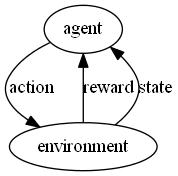
\includegraphics[width=2.5in]{RLDiagram}
\caption{Reinforcement Learning Process}
\label{RLDiagram}
\end{figure}

\section{Methods}
\subsection{State and Action Formulation}
The problem was formulated as a wall following and obstacle avoidance problem in which it was desired to have the robot follow at least $d_{wall} = 0.75 \text{m}$ from a wall, and for the robot to come no closer than $d_{obstacle} = 0.25 \text{m}$ from an obstacle.
The player-stage simulation environment\cite{gerkey_player_2012} (a well known robotics simulation package) was chosen to simulate the actions and environments.  The states were discretized into a minimum left distance, a minimum right distance, and the distance to the closest object.
The actions that the robot could preform was also discretized.  
The robot could either move forward a set velocity (0.1 m/s), or rotate through 360 degrees in 30 degree increments.
The robot could not pick up or move objects.
\subsection{Reward Function}
The reward function is necessary to provide feedback to the robot for being in a certain state.
As the objective is to follow a wall while avoiding obstacles the reward function was designed to penalize the robot (based on a linear scale) on it's distance from the wall or obstacles.   
For example, if the robot was right next the wall (an maximum range of 0.0 m) the reward for that state was -100.  
However, if it was 0.50 m (when the wall following distance was 0.75 m) the reward for that state was only -33.
A similar scheme was employed for the obstacle distances.
It should be noted that terminal states are greater than 1 m from a wall, or with a maximum range of of 0.0 m.
Positive awards were rewarded for each centimeter the robot traveled based on its odometer.
\subsection{SARSA $\lambda$}
The SARSA $\lambda$ algorithm \ref{SARSALambda} was implemented with tables. 
The control policy was initialized to be the previous best (or for the first one a random control policy) and then the robot was released into the world.
Using the $\epsilon$-greedy policy an action was chosen.  The new state was observed, as well as the reward for that state. The control policy was updated to reflect this new change.  This was repeated until a terminal state was reached (i.e. the robot had a collision or strayed too far from the well).
\begin{figure}
\begin{algorithmic}[1]
\State Initialize $Q(s,a)$
\While{For each episode}
    \State Initialize $s$, $a$
    \While{each step of episode}
        \State Take action $a$
        \State Observe $r$,$s'$
        \State Choose $a'$ from $Q(s,a)$
        \Comment{Use $\epsilon$ greedy}
        \State $Q(s,a) \gets Q(s,a) + \alpha \left [r + \gamma Q(s',a')-Q(s,a) \right ]$
        \State $\delta \gets r + \gamma Q(s',a') - Q(s,a)$
    \EndWhile
\EndWhile
\end{algorithmic}
\caption{SARSA $\lambda$ Algorithm}
\label{SARSALambda}
\end{figure}
\subsection{Eligibility Trace}
Eligibility traces serve to address the temporal difference learning problem that arrives from the Monte Carlo formulation of reinforcement learning \cite{szepesvari_algorithms_2010}/
Eligibility traces are used to provide statistics of the attendance of states \cite{szepesvari_algorithms_2010}. 
Each time a state is attended its activity is increased while other states activity is allowed to decay away \eqref{eligibility}.
When added into the SARSA $\lambda$ algorithm the eligibility traces serve to weight states and action that occurred more recently higher while still recording that previous states were visited.
An outline of such an algorithm is presented in \ref{SARSALambdaElig}.
\begin{equation}
\label{eligiblity}
e_t (s,a) = 
\begin{cases}
\gamma\lambda_{t-1}(s), & \text{if} \; s \neq s_t \\
\gamma\lambda_{t-1}(s) +1,& \text{if} \; s = s_t
\end{cases}
\end{equation}

\begin{figure}
\begin{algorithmic}
\State Initialize $Q(s,a)$ and $e(s,a)$
\While{For each episode}
    \State Initialize $s$, $a$
    \While{each step of episode}
        \State Take action $a$
        \State Choose $a'$ from $Q(s,a)$
        \Comment{Use $\epsilon$ greedy}
        \State Observe $r$,$s'$
        \State $\delta \gets r + \gamma Q(s',a') - Q(s,a) $
        \State $e(s,a) \gets e(s,a) +1$
        \ForAll {$s \in S,  a \in A$}
            \State $Q(s,a) \gets Q(s,a) + \alpha \delta e(s,a)$
            \State $e(s,a) \gets \gamma \lambda e(s,a)$
        \EndFor
    \EndWhile
\EndWhile
\end{algorithmic}
\caption{SARSA $\lambda$ Algorithm with Eligibility Traces}
\label{SARSALambdaElig}
\end{figure}

\section{Conclusion}
Reinforcement learning has been proven as a technique of learning a policy necessary to achieve a goal. 
Reinforcement learning (using the SARSA $\lambda$ algorithm) was attempted to be implemented in the player-stage environment in order to teach a robot the optimal policy to avoid walls and to avoid obstacles.
While the particular implementation was not successful at achieving this goal, the general concepts were demonstrated within the framework.
\subsection{Future Work}
As with any implementation that does not converge future work can be made on the convergence of the the algorithm.
Such efforts might focus on a better representation of the state space, perhaps by including more information.Efforts can also be made to improve the reward function, although it is thought that a simple reward function would desired due to the ability to avoid undesired side effects.
Such effects might be teaching the robot incorrect actions by having unintended consequences to the rewards. 
An interesting study could also be completed on training time and the degrees of freedom in the discretization of the state space.
It is thought the training time would increase exponentially with the size of the state space, but this would then allow for the optimal state space parameters for training to be determined.
Finally, the effect of having and training two policies (one for wall following and the other for obstacle avoidance) be investigated.  
It is thought that each individual policy would train faster, but that training the combination of both policies would be difficult to train.
\\
It is proposed for future classes that a code framework be provided with this project. 
This would allow for the students efforts to focus on the actual algorithm rather than the implementation of the states, actions, and how to best store and retrieve them.  If it is desired to have the students think about the implementation of the state and actions, the mini project could be extended to have the student write their own representations, and then a template (or class outlines) be provided for the use in the implementation of the SARSA $\lambda$ algorithm.


% use section* for acknowledgement
\section*{Acknowledgment}
Once again I would like to thank Matthew Lish for his help.  His support and insight is gratefully acknowledgment.


% references section

\bibliographystyle{IEEEtran}
\bibliography{IEEEabrv,Zotero}

% that's all folks
\end{document}


